\subsection{UC16 - Telegram - Interazioni}
		
		%\begin{figure}[t!]
		%	\centering
		%	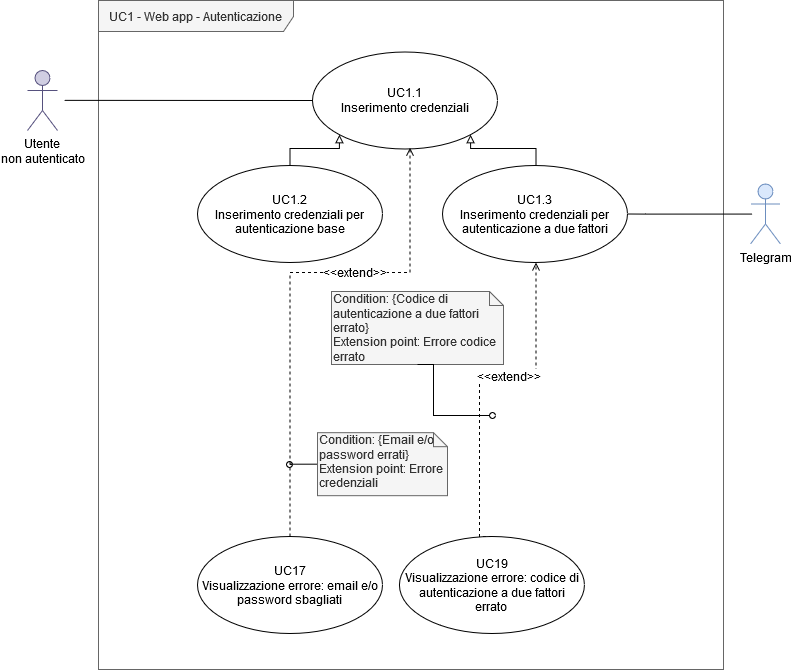
\includegraphics[height=10em]{res/images/uc1}
		%\end{figure}
		
	\begin{itemize}
		\item \textbf{Attori Primari}: Utente autenticato, Moderatore ente.
		\item \textbf{Attori Secondari}: \glock{Telegram}.
		\item \textbf{Descrizione}: Un utente mentre è nell'applicazione di \glock{Telegram} ed ha attiva la schermata di chat con il bot, può eseguire delle interazioni per gestire dispositivi remoti o ricevere informazioni particolari. 
		\item \textbf{Precondizione}: L'utente sta usando l'applicazione di \glock{Telegram} e ha una chat aperta e autenticata con il bot.
		\item \textbf{Postcondizione}: L'utente riceve un messaggio di risposta sulla chat con il bot di \glock{Telegram}.
		\item \textbf{Scenario Principale}:
		\begin{enumerate}
			\item L'utente sta usando l'applicazione di \glock{Telegram} e ha una chat aperta e autenticata con il bot. 
			\item L'utente esegue una interazione con la chat.
			\item L'utente riceve una risposta nella chat del bot.
		\end{enumerate}
	\end{itemize}
	
	\subsubsection{UC 16.1 - Invio comando e ricezione messaggio}

	\begin{itemize}
		\item \textbf{Attori Primari}: Utente autenticato, Moderatore ente.
		\item \textbf{Attori Secondari}: \glock{Telegram}.
		\item \textbf{Descrizione}: Un utente invia un comando nella chat con il bot di \glock{Telegram} e riceve una risposta in base al comando che ha inviato. 
		\item \textbf{Precondizione}: L'utente sta usando l'applicazione di \glock{Telegram} e ha una chat aperta e autenticata con il bot.
		\item \textbf{Postcondizione}: L'utente riceve un messaggio di risposta dopo aver inviato un messaggio sulla chat con il bot di \glock{Telegram}.
		\item \textbf{Scenario Principale}:
		\begin{enumerate}
			\item L'utente sta usando l'applicazione di \glock{Telegram} e ha una chat aperta e autenticata con il bot. 
			\item L'utente invia un comando tra quelli disponibili.
			\item L'utente esegue una interazione con la chat.
			\item L'utente riceve una risposta nella chat del bot.
		\end{enumerate}
		\item \textbf{Specializzazioni}:
		\begin{itemize}
			\item Invio comando /start e ricezione messaggio (UC 16.1.1)
			\item Invio comando /info e ricezione messaggio (UC 16.1.2)
			\item Invio comando /help e ricezione messaggio (UC 16.1.3)
			\item Invio comando /dispositivi e ricezione messaggio (UC 16.1.4)
			\item Invio comando di selezione di un dispositivo e ricezione messaggio con opzioni (UC 16.1.5)
			\item Invio comando di input per un dispositivo e ricezione (UC 16.1.6)
		\end{itemize}
	\end{itemize}

	\subsubsection{UC 16.1.1 - Invio comando /start e ricezione messaggio}

	\begin{itemize}
		\item \textbf{Attori Primari}: Utente autenticato, Moderatore ente.
		\item \textbf{Attori Secondari}: \glock{Telegram}.
		\item \textbf{Descrizione}: Un utente invia un comando nella chat con il bot di \glock{Telegram} e riceve una risposta in base al comando che ha inviato. 
		\item \textbf{Precondizione}: L'utente sta usando l'applicazione di \glock{Telegram} e ha una chat aperta e autenticata con il bot.
		\item \textbf{Postcondizione}: L'utente riceve un messaggio di risposta dopo aver inviato un messaggio sulla chat con il bot di \glock{Telegram}.
		\item \textbf{Scenario Principale}:
		\begin{enumerate}
			\item L'utente sta usando l'applicazione di \glock{Telegram} e ha una chat aperta e autenticata con il bot. 
			\item L'utente invia un comando tra quelli disponibili.
			\item L'utente esegue una interazione con la chat.
			\item L'utente riceve una risposta nella chat del bot.
		\end{enumerate}
	\end{itemize}